\section{Chrip Signal (LFM waveform)}
Chirp는 주파수가 시간에 따라서 증가하거나 감소하는 신호이다. Chirp pulse 의경우 일반적으로 소나 레이저 레이더 및 확산스펙트럼에서 주로 사용이 된다. Chirp 파형의 어원은  새의 짹짹 대는 주파수가 유사해서 짹짹된다는 chrip의 이름을 가진다. LFM\footnote{Linear Frequency Modulation}  signal 이라고도 불린다. 
\subsection{Chrip Signal}
Chirp 파형은 figure와 같이 시간에 따라 주파수가 변화한다. 이때 1차 선형으로 변화하는 LFM과 다른 함수의 형태로 모듈레이션 되는 Nonliear Frequency Modulation으로 나뉜다.\\
    \vspace{-4mm}
    \begin{figure}[!h]\centering
		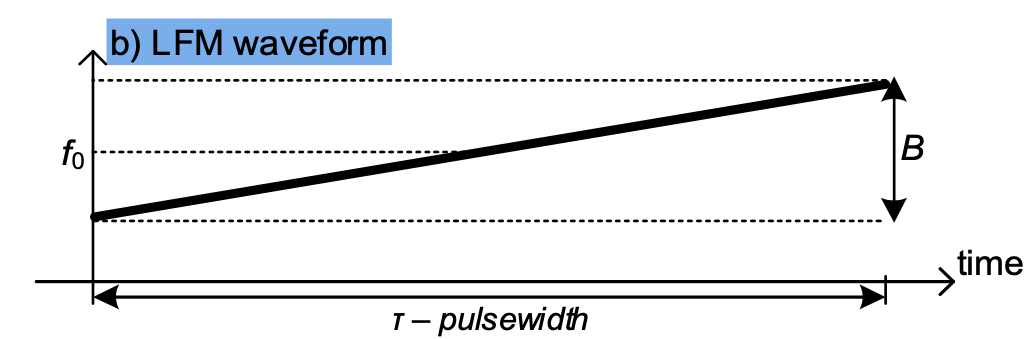
\includegraphics[width=.65\textwidth]{image/week03/1-1.png}
		\caption{\small Frequency change in radar signal}
		\vspace{-10pt}
    \end{figure}
    
예를들어 주파수가 상승하는 up - chirp를 예시로 들자, carrier frequency를 $f_0$라고 하고, $\tau$ 만큼 한개의 펄스가 진행된다면, 순간 주파수는 다음과 같이 표현할 수 있다.
$$
f(t) = f_0 + ut, \quad -\frac{\tau}{2} \leq\ t\ \leq  \frac{\tau}{2}
$$
    \vspace{-4mm}
    \begin{figure}[!h]\centering
		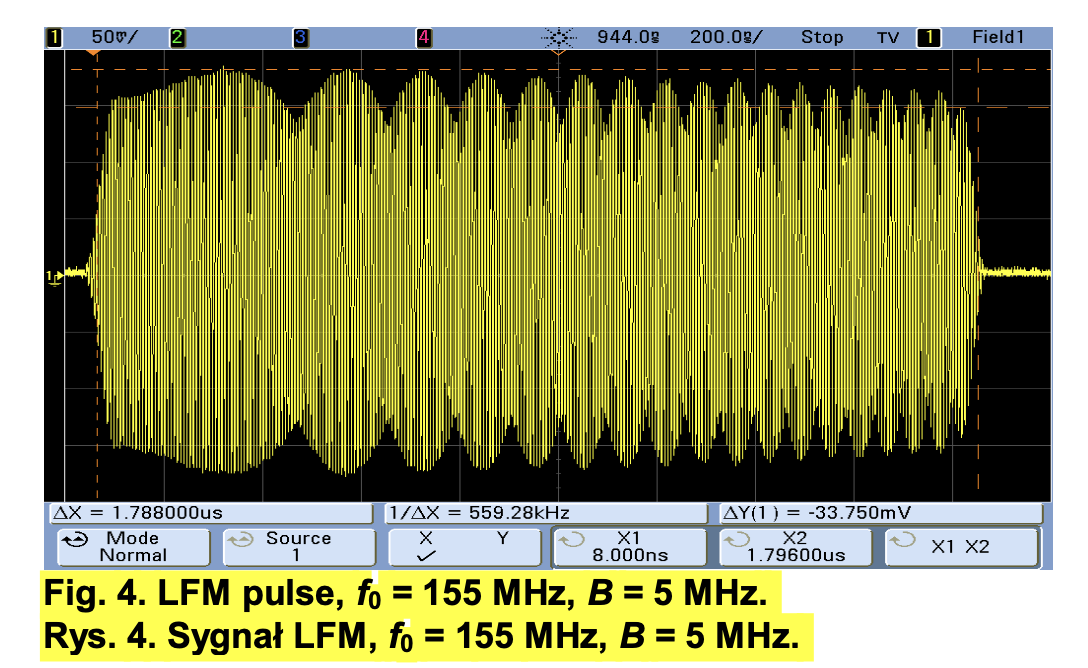
\includegraphics[width=.65\textwidth]{image/week03/1-2.png}
		\caption{\small LFM raadar pulse $a(t) = 1,\ f_0 = 155\ \text{MHZ},\ \phi_0 = 0\ \text{rad},\ \tau= 1.75us, B = 5\text{MHZ}$}
		\vspace{-10pt}
    \end{figure}
\clearpage
다음과 같이 표기할 수 있는 Chirp Signal을 물리적인 안테나로 송신하기 위해서 IQ moudlation을 통해서 ($frequency\ -\ time$) domain 에서 ($amplitude\ -\ time$) domain 의 신호로 변조하여 전송해준다. 
변조된 chirp 신호 (lfm radar pulse)는 아래와 같이 표현할 수 있다. 여기서 $u = B / \tau$ 는 LFM modulation 계수이다. 
$$
s(t) = a(t) \cos(2\pi f(t)+ \phi_0), \quad -\frac{\tau}{2} \leq\ t\ \leq  \frac{\tau}{2}
$$

\subsection{Chrip Radar}
레이더 송신에 사용하는 파형은  FMCW / Stepped Frequency / noise / coded waveform 등이 있다. 그 중에서 가장 많이 사용하는 것이 FMCW 파형이다.\\
FMCW \footnote{FrequencyModulation Continuous Wave} 의 주파수가 모듈레이션되어 있고, 펄스 신호와 같이 특정 시간만 신호가 방사되는 것이 아니라, 계속해서 반복하여 신호를 방사하는 특징을 가진다.  FMCW는 다수의 Chirp signal (LFM 파형)으로 구성되어 있다. 실사용에 사용되는 예시로 자동차 주차보조장치가 있다. 